Even though graph embedding and diagram drawing is a popular subject which has been the topic of articles and research, 
actual open source software which can do such operations is scarce. Algorithms which solve embedding problems have been 
described and implemented since the year 1970. The major impediment for any application which would like to perform 
diagram drawing is actually the diversity and ambiguity of the problem. Apart from performance analysis (time and 
memory consumption), and corectness of the drawing, any other aesthetic appreciation of the result is subjective.
Depending on who the diagram is addressing and which its final scope is, certain styles, connections and layouts are 
appropriate, while others render the final result unasable.

This does not mean that a middle-ground approach does not exist and there are no techniques or conventions which are 
generally accepted as good practice. There are two commonly used open source libraries which provide support for 
drawing diagrams: Graphviz dot\cite{graphvizrelwork} and Eclipse GEF\cite{eclipsegefrelwork}.

\section{Graphviz dot}

\emph{Graphviz dot} is, as described by their own documentation, a command line tool which draws directed graphs as 
hierarchies. It reads its information from text files written in the DOT language and outputs the drawing in 
graphic formats such as GIF(Graphics Interchange Format), PNG(Portable Network Graphics), SVG(Scalable Vector 
Graphics) or PDF(Portable Document Format).

The DOT language input file specifies general information describing the graph. It accepts the definition of three 
main objects: graphs, nodes and edges. A simple graph is described only by its name and a list of nodes and edges.
If the user desires, subgraphs can be defined inside the graph with distinctive characteristics and properties. 
The same can be done for nodes and edges.

\begin{lstlisting}[caption={Simple dot file format}]
digraph G {
	A -> B -> C;
	A -> D;
	A -> E;
	C -> F;
	C -> G;
	D -> F;
	A -> G;
	C -> H;
}
\end{lstlisting}

In terms of implementation, \emph{dot} uses methods such as force directed placing to layout its graphs. Also, its 
layout algorithm presumes graphs are acyclical. This is why dot ensures that all cycles are removed from a graph 
before sending it to the layout routine. 

\begin{lstlisting}[caption={Customized graph dot file representation}]
digraph G {
	size ="4,4";
	main [shape=box]; /*this is a comment*/
	main -> parse [weight=8];
	parse -> execute;
	main -> init [style=dotted];
	main -> cleanup;
	execute -> { make_string; printf}
	init -> make_string;
	edge [color=red]; // so is this
	main -> printf [style=bold,label="100 times"];
	make_string [label="make a\nstring"];
	node [shape=box,style=filled,color=".7 .3 1.0"];
	execute -> compare;
}
\end{lstlisting}

As user-oriented features, the drawings can be manipulated and customized by the user either from a graphical 
interface or by directives specified in the DOT input file. A few examples of such features are: setting dimensions 
and clearance values for node positioning, specifying the direction of edges, label nodes, creatint hyperlinks.

Since it is a command line tool, dot can be integrated with many applications and development environments. From 
custom applications to IDEs, various implementations can use this tool as a means to support drawing diagrams. The 
only requirement is that such an application posseses a means to generate the dot configuration file.

\begin{figure}[ht] \centering
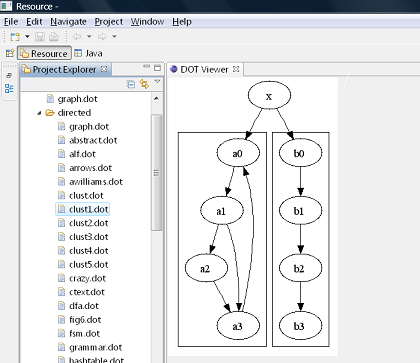
\includegraphics[width=0.45\textwidth]{img/relatedwork/graphviz.png}
\caption{An example of graphviz integrated with the Eclipse IDE.\protect\footnotemark} \end{figure}
\footnotetext{Image taken from \url{http://blog.abstratt.com/}}

\section{Eclipse GEF}

Eclipse GEF(Graphical Editing Framework) provides support for creating graphical editors and views in the Eclipse IDE environment. The graphical 
editors created using GEF allow the user to mainly hand draw any desired graph. All the basic elements required for the task are predefined 
by the underlying library and routing can be performed manually.

Above this basic level, GEF contains classes specialised in layout and connection routing. By default, the library has implementations for 
layout algorithms such as grid layout and tree layout. However, these classes expose API which can be used to create new and more complex 
layout implementations.

\begin{figure}[ht] \centering
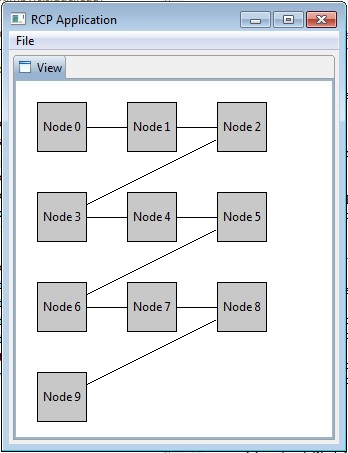
\includegraphics[width=0.35\textwidth]{img/relatedwork/gefexample.jpg}
\caption{Example of a graph viewer implemented using the GEF library.\protect\footnotemark} \end{figure}
\footnotetext{Image taken from \url{http://www.programcreek.com/}}

A notable drawback that GEF presents is the lack of documentation for its API. This may represent a reason why it is not widely 
used, even amongst the Eclipse community. The main sources of information is from articles or community made tutorials, such as 
those of Lars Vogel. Another way of familiarizing oneself with the API and experiencing its capabilities is by running and experimenting 
with the examples suite which comes with the library. These examples showcase typical situations and functionalities step by step through 
simple widgets. While they are educational and helpful for developers, they require an investment of time in order to understand 
the showcased code and functionality.

An extension of Eclipse GEF is Eclipse Zest, which is a visualization toolkit with implementations for different types of graph 
viewers. In essence, a graph viewer is a layout algorithm which specializes in a certain representation of the graph. As 
specified on their homepage, Zest includes a predefined layout package containing algorithms for the following types of 
layouts: Spring, Tree, Radial and Grid. Zest is open to contributions from the community regarding new types of layouts.
Unlike GEF, Zest is does not give the same amount of liberty regarding the representation of nodes. They are static entities, with 
fewer available customizations. Nodes can contain only minimal decorations such as text and an image. This shows that the emphasis 
of this library is on the layout itself.

\begin{figure}[ht] \centering
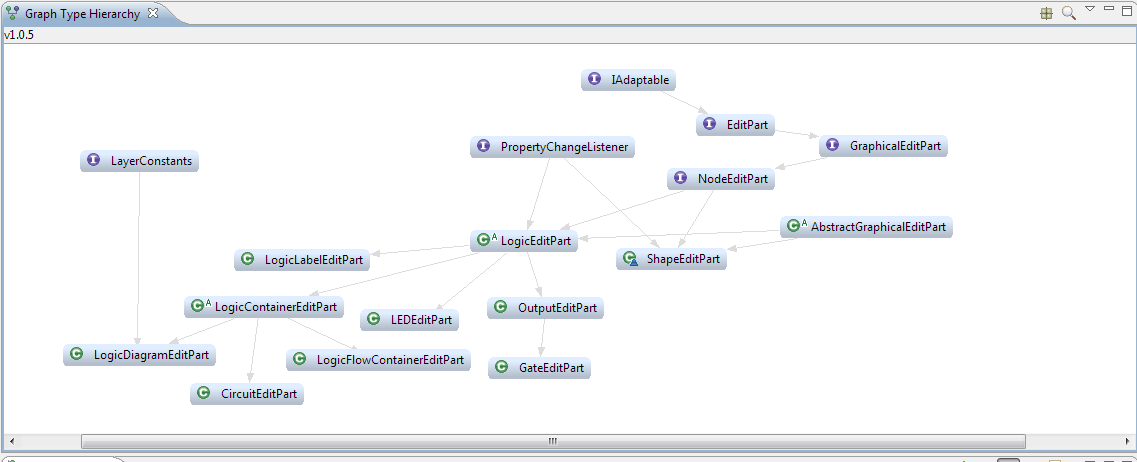
\includegraphics[width=0.85\textwidth]{img/relatedwork/zest.png}
\caption{A graph viewer using Zest radial layout.\protect\footnotemark} \end{figure}
\footnotetext{Image taken from  \url{http://pbwhiteboard.blogspot.ro/}}
